% TODO:
% Decide on CVD or Stroke
% Prepare study design timeline for the mortality study

% general
\documentclass[a4paper,12pt]{article}

% other packages
\usepackage[fleqn]{amsmath}
%\usepackage{geometry}

% graphics
\usepackage{graphicx}
\graphicspath{{./plots/}}
\usepackage[font=small,labelfont=bf]{caption}
\usepackage{float}

% landscape and longtables
\usepackage{pdflscape}
\usepackage{longtable}

% hebrew
\usepackage{fontspec}
\usepackage{polyglossia}
\usepackage[utf8x]{inputenc}
%\usepackage{hebfont}
%\newfontfamily\hebrewfont[Script=Hebrew]{Miriam Mono CLM}
%\newfontfamily\hebrewfont[Script=Hebrew]{Frank Ruehl CLM}
\newfontfamily\hebrewfont[Script=Hebrew]{David CLM}
\setmainlanguage{english}
\setotherlanguage{hebrew}

% bib
\usepackage[backend=bibtex]{biblatex}
\addbibresource{bibtex/proposal.bib}

% spacing
\usepackage{setspace}
\linespread{1.25}
\setlength{\parskip}{\medskipamount}
\setlength{\parindent}{0pt}

% appendices
\usepackage[toc,page]{appendix}

% csv
\usepackage{csvsimple}

\begin{document}
	
	\title{PhD Proposal}
	\author{Noam Barda}
	\maketitle
	
	\tableofcontents
	\newpage
	
	\section{Abstract}
	
		\subsection{Background}
		Since the early 1990s, and more so in the last few years,  multivariate risk models have been created to estimate patients' risk for different diseases over different time spans (e.g. \cite{Wilson1998,Conroy2003,DAgostino2008}). These models are used to identify patients at risk and are capable of exact risk quantification over time\cite{Goff2014}. Through their many variations, these risk models are included in different guidelines and occupy an important place in both primary prevention and diagnosis of different diseases\cite{Graham2007,Goff2014}.
	
		Such multivariate risk models have several characteristics:
		\begin{itemize}
			\item Their development has traditionally required extensive input from domain experts (clinicians) for the choice of predictors.
			\item Their performance is highest in the population used to develop them and is reduced on populations that are genetically or otherwise different\cite{DAgostino2001,Bastuji-Garin2002,DeFilippis2015}.
			\item They are traditionally based on classic biostatistical models, usually logistic and Cox regression.
		\end{itemize}
	
		\subsection{Goals}
		We intend to pursue three goals in this thesis:
		\begin{itemize}
			\item Recent advances in machine learning allow for a new approach to medical risk modeling\cite{Obermeyer2016}. Contrary to the classic approach that emphasizes domain knowledge for the pre-specification of risk factors, novel methods rely instead on sophisticated algorithms being presented with thousands of candidate variables and selecting the relevant ones by themselves. These variables are then used for the actual model building\cite{Weng2017}. Such technologies allow a more standardized "one-size fits all" approach to risk modeling, utilizing a single comprehensive database with different outcomes\cite{Rajkomar2018}. We intend to establish a generic prediction framework allowing the standardized construction of validated predictive models for any outcome.
			\item Two medical domains will be chosen: Cardiovascular Disease (CVD) and short-term mortality. In both domains, a predictive model will be developed using the above-mentioned algorithm and then compared to existing models from the literature. This will serve two purposes: One, it will illustrate that a model developed in such an automated process can outperform existing models. Two, it will serve to externally validate the performance of existing models on the Israeli population. No such external validation exists, to the best of our knowledge.
			\item With a CVD model developed, we will simulate the likely effects of using such a model in the population in regard to CVD prevention, based on existing guideline recommendations\cite{Goff2014}.
		\end{itemize}
	
		\subsection{Methods}
		The generic prediction framework will make use of a sparsity inducing algorithm fed with the majority of the variables in the Clalit's electronic health record. The algorithm will then choose the appropriate variables and construct a model. The model will first be tuned on a validation set and then evaluated on a test set.
		
		To perform external validation and comparison, two leading CVD models and two leading one-year-mortality will be selected and recreated on the Clalit's database. The models will be compared in their original population composition and on a common sample corresponding to the population on which we intend to simulate our intervention.
		
		The simulated CVD intervention will examine a retrospective cohort of patients, and will utilize existing knowledge regarding the mortality reduction attributed to statin and aspirin use to simulate the 10-year-outcomes of this cohort had existing guidelines been adhered to.

		\subsection{Importance}
		A generic prediction framework will allow easy construction of validated predictive models of high quality, with the variable selection portion affording possible biological insight.
				
		External validation of CVD and mortality risk models, currently in wide use and integrated into guidelines, is of vital importance\cite{Moons2012}.
		
		Simulating  the intervention will allow us to gauge the potential effectiveness of interventions based on such risk models. Such interventions are becoming more and more possible with widespread electronic health record availability.
	
	
	\section{Hebrew Abstract}
	
	\begin{hebrew}
		\subsection*{רקע}
		מתחילת שנות ה-90 החלה, ובשנים האחרונות גברה, יצירתם של מודלים רב-משתניים לחישוב סיכון למחלות שונות(לדוגמה \cite{Wilson1998,Conroy2003,DAgostino2008}). מודלים אלו משמשים לזיהוי חולים בסיכון, ומאפשרים כימות מדויק של הסיכון לאורך שנים רבות\cite{Goff2014}. כיום, בצורותיהן השונות, מודלים אלו כלולים בקווים המנחים של ארגונים מקצועיים רבים, ולהם מקום חשוב הן במניעה הראשונית והן באבחנה של מחלות \cite{Graham2007,Goff2014}.
			
			למודלים אלו מספר מאפיינים:
			\begin{itemize}
				\item פיתוחם דרש באופן מסורתי התייצעות נרחבת עם מומחי תוכן (קלינאים), על מנת שאלו יספקו את המידע הנדרש בנוגע למשתנים הנדרשים לחיזוי התוצא.
				\item ביצועיהם של מודלים אלו מיטבי כאשר משתמשים בהם באוכלוסיות עליהם פותחו, ופוחת באוכלוסיות השונות מאוכלוסיות אלו מבחינה גנטית או אחרת\cite{DAgostino2001,Bastuji-Garin2002,DeFilippis2015}.
				
				\item המודלים מבוססים ככלל על שיטות ביוסטטיסטיות מסורתיות, בפרט על רגרסיה לוגיסטית ורגרסיית קוקס.
				
			\end{itemize}
				
		\subsection*{מטרות}
			כוונתנו להשיג שלוש מטרות בתזה זו:
			\begin{itemize}
				\item חידושים מודרניים בלמידה חישובית מאפשרים גישות חדשות למידול סיכון רפואי\cite{Obermeyer2016}. בניגוד לגישה הקיימת, המבוססת על שימוש בידע תחומי לפירוט-מראש של גורמי הסיכון, גישות מודרניות מתירות לאלגוריתם החישובי, המוזן עם מאות משתנים אפשריים, לברור מביניהם את המשתנים הרלוונטיים בכחות עצמו\cite{Weng2017}. לאחר מכן, משתנים אלו משמשים לבניית המודל עצמו. טכנולוגיות אלו מאפשרות גישה יותר אחידה למידול סיכון, המשתמשת בבסיס נתונים נרחב יחיד עם תוצאים שונים\cite{Rajkomar2018}. אנו מתכוונים ליצור בסיס נתונים שכזה על מנת לבנות מודל סיכון חדש  לשבץ, אשר ישמש בעבודה זו.
				\item שני תחומים רפואיים יבחרו: חיזוי מחלה קרדיווסקולרית ותמותה קצרת-טווח. בשני התחומים ייבנה מודל חיזוי באמצעות האלגוריתם דלעיל ויושווה למודלים קיימים בספרות. השוואה זו תשרת שתי מטרות: האחת, להדגים שמודל שפותח באופן אוטומטי שכזה יכול שיהיו ביצועיו עדיפים על מודלים קיימים.  השניה, תיקוף חיצוני של המודלים הבינלאומיים על גבי האוכלוסיה הישראלית. למיטב ידיעתנו, תיקוף שכזה טרם בוצע.
			\end{itemize}
		
		\subsection*{שיטות}
			השלד לחיזוי גנרי יעשה שימוש באלגוריתם המבצע בחירת משתנים כחלק מפעולתו. אלגוריתם זה יוזן עם מרבית המשתנים הזמינים בבסיס הנתונים של קופ"ח כללית, מהם יבחר המשתנים הרלוונטיים בהם יעשה שימוש לבניית מודל. המודל יכוונן על גבי אוכלוסיית פיתוח וייבדק מול אוכלוסיית בדיקה.
			
			על מנת לבצע תיקוף חיצוני והשוואה, שני מודלים מובילים לחיזוי CVD ושני מודלים מובילים לחיזוי תמותה בשנה הקרובה ייבחרו מהספרות וייבנו מחדש על גבי בסיס הנתונים של הכללית. המודלים יושוו הן בהרכב האוכלוסיה המקורי בו נבנו והן בהרכב האוכלוסיה בו אנו עתידים לדמות התערבות.
			
			סימולציית ההתערבות תבחן עקבה רטרוספקטיבית , ובאמצעות ידע קיים בנוגע להפחתת התמותה המיוחסת לשימוש בסטטינים ובאספירין, תדמה התוצאים ל-10 שנים  של עקבה זו  באם הקוים המנחים הקיימים היו מקויימים כלשונם, לפי המודלים הקיימים ולפי המודל החדש.
			
		\subsection*{חשיבות}
			מסגרת לחיזוי גנרי תאפשר בניית מודלים מתוקפים ובאיכות גבוהה לחיזוי מחלות שונות, ועצם תהליך בחירת המשתנים יכול שיאפשר תובנות ביולוגיות.

			תיקוף חיצוני של מודלים לחיזוי מחלה קרדיווסקולרית, המצויים בשימוש רחב ומשולבים בקווים המנחים, הוא בעל חשיבות מכרעת\cite{Collins2015}.
			
			סימולציית ההתערבות תאפשר לנו לשפוט את האפקטיביות של התערבויות המבוססות על מודלים שכאלו. לדבר חשיבות מוגברת היות שהתערבויות אלה הופכות אפשריות יותר ויותר עם הופעתם של בסיסי נתונים גדולים המבוססים על תיקים ממוחשבים.
		
	\end{hebrew}
	
	\section{Aim of the Thesis}
	The main aim of this thesis is to design, implement and evaluate an algorithm to develop multivariate predictive models based on Clalit Health Services' (CHS) electronic health record based database.
	
	The aforementioned goal will require three steps:
	\begin{description}
		
		\item[Model Development] A modern and novel approach to develop risk models based on Electronic Health Record (EHR) data will be developed. The full details of this approach will be detailed below, under "Research Methodology", but briefly, it will require no preliminary domain expertise, instead utilizing modern methods to simultaneously choose variables and create the model based on them.
		
		\item[Model Evaluation] The above-mentioned approach will be used to construct two risk models: Cardiovascular Disease (CVD) 10-year prediction and 1-year mortality. The merits of these models will be tested by comparing them to leading existing models from the literature. This evaluation will comprise a comprehensive test of these models' performance in both their original population composition and in a shared population with the characteristics we intend to use in our intervention.
		
		\item[Simulated Intervention] The CVD model will be used to simulate an intervention based on a historic cohort of patients from the CHS' database. The true outcomes, the predicted outcomes based on existing models and the predicted outcomes based on our models will be compared.
		
		Based on these aims, we hypothesize that:
		\begin{enumerate}
			
			\item That using less pre-specification of risk factors, and allowing a computerized algorithm to select risk factors in an autonomous fashion, will enable detection of novel risk factors, whose inclusion in future risk models will improve their performance.
			
			\item That a model developed in such fashion will outperform traditional risk models.
			
			\item That the advantages of such a model will have the potential to improve patient outcomes if used in a population-wide intervention based on EHR data.
			
		\end{enumerate}
		
	\end{description}
	
	\section{Importance and Background}
	
	We will survey the pertinent background for each step in turn, highlighting the gap in existing knowledge to which we seek to contribute.
	
		\subsection{Part I}
		
		\subsubsection{Methodology of Traditional Risk Models}
		
		For traditional medical risk models, two design decisions are ubiquitous\cite{Weng2017}:
		\begin{enumerate}
			\item They are based on traditional biostatistical methodology such as generalized linear and cox models.
			\item They rely heavily on the use of domain expertise to identify relevant risk factors.
		\end{enumerate}
		
		Informally described, we could say that the model is tasked to estimate the relative weights of risk factors, themselves independently pre-identified by domain experts.
		
		\subsubsection{Generalized Linear Models}
		
		Generalized linear models (GLMs) are parametric models that are generalizations of ordinary linear regression, allowing outcome variables to have non-normal error distributions\cite{Nelder1972}.
		
		While classic linear regression follows the form:
		\begin{equation*}
		E[Y] = x^t \beta
		\end{equation*}
		
		GLMs have the form:
		\begin{equation*}
		E[Y] = g^{-1} (x^t \beta)
		\end{equation*}
		
		With g being the link function connecting the linear predictor space with the outcome space.
		
		For example, logistic regression uses the logit function as the link, $ \mu = \frac{\exp (x^t \beta)}{1 + \exp (x^t \beta)} $, while linear regression uses the identity function.
		
		The model then uses a loss function, usually maximum likelihood, to estimate the coefficients of the model. Under certain assumptions, these coefficients can have epidemiological interpretations, such as the coefficients of logistic regression being interpreted as odds ratio of an exposure for a given outcome. The model can also be used for prediction, disregarding all such assumptions.
		
		\subsubsection{Cox Proportional Hazards}
		
		The cox model is a survival analysis model (that is, it uses a compound outcome of time-to-event data) that is semi-parametric. A baseline hazard ($ \lambda_0 $) is estimated non-parametrically from the data, while a parametric linear hazard model is estimated in parallel\cite{Cox1972}.
		
		The overall hazard model is thus $ \lambda(t) = \lambda_0(t) \cdot x^t \beta $. The hazard itself is a somewhat elusive term rooted in calculus, representing the probability of death at a certain infinitesimal time window assuming survival up to that point. Survival is then one minus the integral of the hazard over time.
		
		Similar to GLMs, the coefficients are estimated using a process of maximum likelihood (dubbed partial likelihood in the context of Cox regression), and under strict assumptions have the interpretation of hazard ratios, similar to odd ratios.
		
		The assumptions for cox regression warrant special mention. While the assumption of linearity is similar to GLMs, cox proportional hazards also assumes proportionality - that is, that the hazard ratio between risk factors remains constant over time. This is a very strong assumption that does not always hold. It should be mentioned that some models circumvent this assumption at the cost of complexity and loss of interpretability. Just as before, the model can also be used for prediction, disregarding all assumptions.
		
		\subsubsection{Parametric Vs. Non-Parametric Models}
		Parametric models, such as those described above, summarize the data with a set of parameters of fixed size that is independent of the number of training examples. This has the advantage of simplicity, interpretability and speed, but also leads to biases in prediction if the "true" population model is different than the chosen model.
		
		Non-parametric models make no such assumptions about the structure of the target function they seek to learn. This requires far more data for accurate training, and does not allow interpretation of coefficients using terms such as odd ratios, but does afford more predictive accuracy when sufficient data exists\cite{Russell2002}.
		
		\subsubsection{The Rise of AI and Machine Learning}
		
		In recent years the fields of machine and statistical learning have seen a tremendous rise\cite{Obermeyer2016}. this growth in machine learning, including predictive modeling, has occurred thanks to three main factors\cite{Shalev-Shwartz2014}:
		\begin{itemize}
			\item A large increase in the amount of accessible data.
			\item The development of new algorithms and methods.
			\item An increase in computation power.
		\end{itemize} 
		These new methods have several defining characteristics, including:
		\begin{itemize}
			\item The use of a wider range of algorithms, not limited to generalized linear models.
			\item Less reliance on domain expertise, in essence allowing the algorithm to both find the main risk factors and to estimate their respective weights.
			\item The need for larger sample sizes, to allow the more complex modeling to occur successfully.
		\end{itemize}
		To date, these methods have yet to gain wide-acceptance in medical practice\cite{Obermeyer2016,Deo2015}.
		
		\subsubsection{Black-Box Vs. White-Box Models}
		While there are obstacles from many different domains to the integration of machine learning approaches in medicine: psychological, legal, regulatory and others, one overarching concern is the preeminence of black-box models in machine learning\cite{Price2015}.
		
		Broadly defined, black-box models are models whose results cannot be readily explained. For example, a logistic regression result can be fairly easily reasoned about: baseline risk was x\%, and a certain combination of variables increased the risk by y\% more. The same cannot be said for most models used in modern machine learning, including neural networks and tree-ensemble models. These models generate a result that is a complex non-linear function of their inputs, and one cannot easily explain why a specific patient got a risk of x\%, while another got y\%.
		
		Beyond the legal and psychological difficulty this creates (how does one explain, to oneself and others, a decision based on unclear reasoning?), it also introduces the possibility of discrimination. The algorithm could choose to optimize for one (majority) population, while neglecting other (minority) populations\cite{Hebert-Johnson2017}. This fascinating area of research falls under the more general notion of algorithmic fairness, more widely studied in other non-medical fields\cite{Corbett-Davies2017}, and is beyond the scope of this thesis.
		
		\subsubsection{Electronic Health Record based Observational Studies}
		
		Most medical risk models in wide-use were developed based on specialized cohort studies\cite{Goldstein2016}. This has the known advantages of cohort studies, most notably the accurate definition of exposures and outcomes, but is expensive and time-consuming, and by definition only allows inclusion of risk factors that were decided on in advance and measured as part of the study. On the other hand, with the larger availability of EHR data, risk models developed on such data have risen in amount. These models have the known disadvantages of EHR data (first of which are the non-standardized definitions), but offer a wealth of information that in certain cases, including the case in Israel\cite{Lovis2015}, encompasses the full extent of a patient's encounters with the health system\cite{Goldstein2017}.
		
		\subsubsection{The Gap and our Thesis}
		
		We suggest using the unique availability of widely encompassing EHR data with large historic depth, coupled with modern statistical learning methods, to develop a generic method for generation of risk models based on the Clalit's EHR.
		
		This method will make use of most available EHR data, and will require no pre-specification of risk factors, instead allowing the algorithm to ascertain the relative importance of the different factors by itself. Not only will this allow the creation of accurate risk models, it will also provide a way to automatically identify associations that exist in the EHR and could present novel risk factors and biological pathways.
		
		We will then use this method to develop 2 specific models to predict CVD and mortality. As this model will make use of large portions of the EHR data and will be purposely built on the Clalit's population, it is likely to perform well.
		
		\subsection{Part II}
		
			\subsubsection{Epidemiology of Cardiovascular Disease}
			
			In its usual definition, cardiovascular disease (CVD) includes several disease categories\cite{WHO2017}:
			\begin{enumerate}
				\item Coronary Heart Disease
				\begin{enumerate}
					\item Myocardial Infarction
					\item Angina Pectoris
					\item Heart Failure
					\item Coronary death
				\end{enumerate}
				\item Cerebrovascular Disease
				\begin{enumerate}
					\item Stroke (Thrombotic and Hemorrhagic)
					\item Transient Ischemic Attack
				\end{enumerate}
				\item Peripheral Artery Disease
				\item Aortic Disease
				\begin{enumerate}
					\item Atherosclerosis
					\item Aneurysm
				\end{enumerate}
				\item Rheumatic Heart Disease
				\item Congenital Heart Disease
				\item Venous Thromboembolism
				\begin{enumerate}
					\item Pulmonary Embolism
					\item Deep Vein Thrombosis
				\end{enumerate}
			\end{enumerate}
		
			CVD is very common. Lifetime risk for people aged 30 with no prior cardiovascular disease approaches 50 percent\cite{Rapsomaniki2014}, with coronary heart disease being the most common specific diagnosis\cite{Benjamin2017}.
	
			While the rates of cardiovascular disease in general have declined in developed countries over the last 30 years\cite{Koton2014,Vangen-Loenne2017}, they remain significant public health problems, being the second most common cause of mortality and third most common cause of disability worldwide\cite{Lozano2012}. The statistics in Israel are similar\cite{ICDC2017}.
			
			Among diseases with such a significant public health impact, cardiovascular disease stands out in two ways. First, its risk factors are well understood, with 90\% of its population-attributable-risk caused by nine risk factors. It's also a very preventable disease, as these risk factors are mostly preventable\cite{Yusuf2004,ODonnell2016}: Smoking, dyslipidemia, hypertension, diabetes, etc.
			
			\subsubsection{History of Multivariate Risk Models}
		
			These unique characteristics have made CVD the main outcome in risk models, when such models began to enter clinical practice in the 1990s\cite{Wilson1998,NationalCholesterolEducationProgramNCEPExpertPanelonDetection2002,Conroy2003,Hippisley-Cox2007,DAgostino2008,Hippisley-Cox2008,Goff2014}. Still the most notable of said risk models is the Framingham risk model family, developed on a US population in Massachusetts, Boston\cite{Wilson1998}, and the SCORE risk model, developed in 2003 on a European population\cite{Conroy2003}.
			
			Perhaps more important that their mere existence, is that these models have made their way into widely-accepted international guidelines, with their use mandated in routine clinical care. Two examples we'll cite are the use of these risk models in deciding on Statin therapy\cite{Goff2014} and their use in deciding on anti-platelet therapy\cite{Bibbins-Domingo2016}, both for primary prevention of CVD.
			
			While CVD prediction was the bedrock for clinical risk models, they have since spread to encompass a large variety of diseases categories\cite{Kanis2008,Kansagara2011}, and have found use not only in prediction, but also in diagnosis\cite{Usher-Smith2016}. This increasingly important place taken by risk models has brought about the publication of guidelines designed to regulate and improve their creation\cite{Collins2015}. As estimating the probability for existing and future disease is a significant portion of the clinical process\cite{Moons2009}, and as this task can in large parts be automated, it seems likely that risk models will gain an increasingly important place in the medical practice.
			
			\subsubsection{Limitations of Risk Models}
		
			Naturally, risk models are developed on a specific population, whose data is available to the researchers developing the model. As patients differ in a variety of ways (both genetic and environmental), and even such basic things as lab methods and disease definitions differ in different areas, models tend to function better when used on the population on which they were developed\cite{DAgostino2001,Bastuji-Garin2002}.
			
			Recent models have tried to deal with this problem by including more ethnically varied populations\cite{DeFilippis2015} or recalibrating the model for each new population\cite{Kanis2008}, but such efforts are limited to specific risk models, and even then have only been partially successful\cite{Dagan2017}. As one specific Israeli example, this phenomenon was observed in a recent publication that illustrated significant mis-calibration for osteoporosis prediction models that are in wide clinical use and incorporated into guidelines\cite{Dagan2017}. As the probabilities generated by the model eventually help determine the proper interventions to perform, according to respective guidelines, such mis-calibration could invalidate the use of the model, making external validation an important endeavor\cite{Moons2012}.
			
			\subsubsection{The Gap and our Thesis}
		
			Though the risk scores are currently used in common medical practice, external validation of international CVD risk models for the Israeli population has yet to be performed, and recommendations on which model to use are based on expert opinion\cite{Bitzur2015}.
			
			We will, as part of our effort, externally validate widely used risk models for the prediction of CVD risk on the Israeli population. This could help decide which model has the best performance, and if all such models' performance is deemed unsatisfactory, this will have significant consequences for guidelines and practices based on said models.
			
			We will then compare said models to our own internally developed model.
			
		
		\subsection{Part III}
		
			\subsubsection{Traditional Aim of Risk Models}
			
			Outside of the realm of medicine, risk models are used for great many purposes: deciding which customers are likely to default on loans, deciding which credit card deals are fraudulent, deciding which customers are likely to churn, etc.
			
			Within the realm of medicine, the use of risk models is fairly consistent. When deciding on some intervention to lower some risk (e.g. statins for CVD), one has to always remember that interventions have risks themselves (e.g. rhabdomyolysis from statins). For any utility one mentally assigns lower CVD risk and higher rhabdomyolysis risk (in our example), the prescription of statins is more warranted if the baseline risk for CVD is higher. This is intuitive and simple - one does not walk around wearing a Hazmat suit if one is not in the immediate vicinity of hazardous materials (presumably because its hot within such suits).
			
			With this logic in mind, risk models are constantly used, consciously and subconsciously, when deciding on diagnostic and therapeutic interventions. Consciously, for example, when deciding on aspirin and statins for CVD risk\cite{Goff2014,Bibbins-Domingo2016}, bisphosphonates for osteoporosis risk \cite{Jeremiah2015} or CT angiogram for pulmonary thromboembolism risk\cite{Wells2001}. Subconsciously, for example, when deciding whether to refer a patient suspected of pneumonia to a chest x-ray.
			
			\subsubsection{The Way Risk Models are Used}
			
			For several reasons, utilizing risk models for these aims requires the direct involvement of a treating physician:
			\begin{enumerate}
				\item The different risk models require knowledge of a wide variety of clinical factors, including lab results that most patients are not expected to know themselves.
				\item The decisions to be made can only be made by a physician. A patient cannot prescribe statins to himself.
			\end{enumerate}
			
			And so the use of such model has mostly been limited to physicians. To make use of these risk models, the physician, usually the primary care physician, is required to the fill in the different covariates based on the patient's health record, communicate the results to the patient, and advise on whatever intervention is mandated to mitigate the risk.
			
			It should be said that this entire time consuming act is expected to occur in an already time-strained primary care encounter\cite{Konrad2010}.
			
			\subsubsection{Empowering Patients to Control Risk Factors}
			This physician-led approach to health maintenance is by no means the only one. Complementary to it is the idea of self-care, the enlightening definition for which we'll copy from the WHO verbatim: \textbf{"Self-care in health refers to the activities individuals, families and communities undertake with the intention of enhancing health, preventing disease, limiting illness and restoring health. These activities are derived from knowledge and skills from the pool of both professional and lay experience. They are undertaken by lay people on their own behalf, either separately or in participative collaboration with professionals"}\cite{Organization1984}.
			
			These ideas are of particular importance in the field of CVD management and prevention as\cite{Riegel2017}:
			\begin{itemize}
				\item CVD is very prevalent, and management of its many risk factors, signs and symptoms could "drown" modern primary care.
				\item CVD has many risk factors that can be addressed independently by patients with little-to-no physician involvement (e.g. by physical activity, proper diet, smoking cessation, etc.)
			\end{itemize}
		
			\subsubsection{Bridging Self-Care and Risk Modeling}
			
			Naturally, knowledge of one's health status is paramount to one's management of it. Such plans as the American Heart Association's "know your numbers" are geared towards encouraging patients to question their family physicians regarding several basic clinical markers and lab results\cite{Riegel2017}. While this approach also requires the direct involvement of the treating physician, this requirement is brought about by the structure of the American health care system and availability of information, and is not inherent in the problem.
			
			Whether such interventions are effective is an open question. While the American health care system does not allow easy appraising of the effectiveness of interventions such as "know your numbers", other health care systems do. A study conducted in Australia found that patients advised regarding their own hypertension in incidental pharmacy visits, had improved knowledge of hypertension management and sought health-care more often\cite{Cadilhac2015}.
			
			\subsubsection{The Gap and our Thesis}
			
			We suggest that the structure of the Israeli health care system is ideal for performing and evaluating an intervention based on promoting CVD prevention self-care.
			
			In this thesis, the risk model will be presented directly to the patient, with the different covariates extracted seamlessly from the patient's electronic health record. The presentation will include visual queues regarding the normal range of risk factors and an ability to view the effect of altering specific risk factors.
			
			It will also include personalized recommendations for the reduction of risk based on the patient's characteristics, suggesting self-care options when such options exist, and recommending physician contact when such contact is warranted.
	
	\section{The Novelty of the Thesis}
	
	All aforementioned aspects of the thesis contain measures of novelty to them:
	
	\begin{itemize}
		
		\item We propose that the methodology by which the model will be developed, and specifically its wide applicability, requiring little human intervention and pre-processing, offers significant advantages. The ability to identify risk factors and construct models for a wide variety of pathologies, some of which "unmapped" in regard to their primary risk factors, offers a promise of better understanding and more focused interventions to prevent these diseases.

		\item External validation of existing risk models is of utmost importance\cite{Moons2012}, as these models are used constantly as part of existing guidelines (e.g. the American Heart Association's pooled risk model and Statin treatment\cite{Goff2014}, FRAX and Osteoporosis treatment\cite{Kanis2008}). This is especially true, as previous external validation studies have at times documented significant mis-calibration\cite{Bastuji-Garin2002,Dagan2017}, that would make treatment decisions based on the models problematic.
		
		\item Population wide EHR-data based interventions using predictive risk models have yet to be implemented, to the best of our information. Illustrating the advantages of such interventions, specifically with the rising availability of EHR data, is of significant importance.
		
	\end{itemize}
	
	\section{Published Work}
	
	The epidemiological characteristics of CVD in general and of stroke in particular are well understood\cite{Koton2014,Vangen-Loenne2017}, and the dominant risk factors in the population well mapped\cite{Yusuf2004,ODonnell2016}. This is true both in the developed and in the developing world\cite{Lozano2012}. It is also true in Israel\cite{ICDC2017}.
	
	The increasingly central role filled out by risk prediction models in medicine has been observed\cite{Moons2009}, as have the challenges of developing such models based on Electronic Health Record (EHR) data\cite{Goldstein2016,Goldstein2017}. This rapid rise in the number of risk prediction models has led to the writing of specific guidelines on how to develop such risk models and report their results\cite{Collins2015}.
	
	Many CVD risk models have been developed in the last 30 years, most prominent of which are the Framingham\cite{Wilson1998,NationalCholesterolEducationProgramNCEPExpertPanelonDetection2002,DAgostino2008,Goff2014}, SCORE\cite{Conroy2003} and Qrisk\cite{Hippisley-Cox2007,Hippisley-Cox2008} families of models.	Two of these model families also offer a stroke-specific model\cite{Wolf1991,DAgostino1994,Hippisley-Cox2013}.
	
	Risk models have been incorporated into guidelines for the prevention, diagnosis and treatment of varying conditions. Specifically for CVD prediction, these risks help decide on cholesterol lowering treatment, anti-platelet treatment and more generally, the intensity of follow-up\cite{NationalCholesterolEducationProgramNCEPExpertPanelonDetection2002,Graham2007,Goff2014,Bibbins-Domingo2016}.
	
	Models' tendency to under-perform when the target population is changed is widely recognized\cite{DAgostino2001,Bastuji-Garin2002,DeFilippis2015} and accordingly, the importance of external validation of models prior to their use in new population is recommended\cite{Moons2012}. External validation of CVD models has been performed in several populations\cite{DAgostino2001,Bastuji-Garin2002,DeFilippis2015}, though not in the Israeli population\cite{Bitzur2015}. This is in contrary to, for example, Osteoporosis\cite{Dagan2017}.
	
	Much has been written on the advent of AI in general and machine learning in particular. In a relatively short time span, these technologies have penetrated large parts of the domains of modern life, and continue to do so in increasing force\cite{Ng2017}.
	
	That this process has been relatively slow in medicine is also widely recognized, and many efforts now exist to better incorporate such technologies in health-care\cite{Obermeyer2016}. Specifically for risk prediction models, recent literature has emerged that details attempts at developing more generic risk models, though different than the idea proposed here both in method and in goal\cite{Rajkomar2018}.
	
	\section{Research Methodology}
	We will elaborate on the following for each of the three parts:
	\begin{itemize}
		\item Planning, including population definition and variables.
		\item Data extraction.
		\item Descriptive statistics.
		\item Modeling and inferential statistics.
	\end{itemize}

	\subsection{Planning}
	
		\subsubsection{Part I}
		Our models will be developed on the following population.
		
		CVD Model:
		Inclusion:
		\begin{itemize}
			\item Ages 30-90.
			\item At least 1 year of continuous membership in the Clalit prior to the index date.
			\item Continuous membership until the study end date or until death.
		\end{itemize}
		Exclusion:
		\begin{itemize}
			\item Past CVD event (Stroke, Myocardial Infarction, Peripheral Artery Disease).
		\end{itemize}
		
		As is the standard for cardiovascular disease risk models, our model will predict disease for 10 years after the index date. The index date will be set at 1/6/2007, and follow up will persist until 1/6/2017, as illustrated in the following design diagram.
		
		\begin{figure}[h]
			\centering
			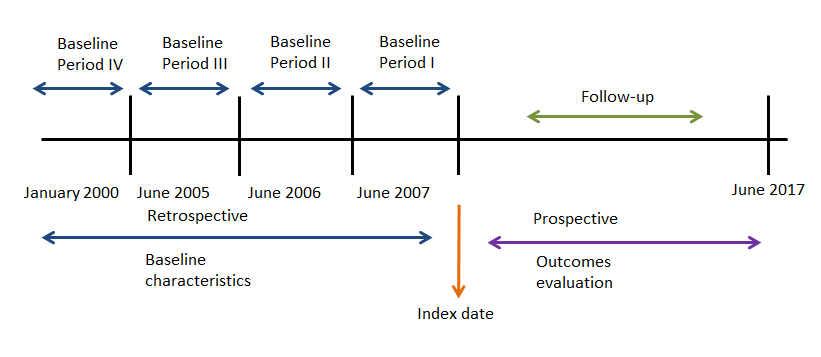
\includegraphics[width=\textwidth]{prelim-results/Panpredictor/timeline1.png}
			\caption{Study Design Timeline}
		\end{figure}
	
		Mortality Model:
			Inclusion:
		\begin{itemize}
			\item Ages 50-90.
			\item At least 1 year of continuous membership in the Clalit prior to the index date.
			\item Continuous membership until the study end date or until death.
		\end{itemize}
		Exclusion:
		\begin{itemize}
			\item None.
		\end{itemize}
		
		Our model will predict all-cause mortality for 1 year after the index date. The index date will be set at 1/6/2016, and follow up will persist until 1/6/2017, as illustrated in the following design diagram.
		
		\begin{figure}[h]
			\centering
			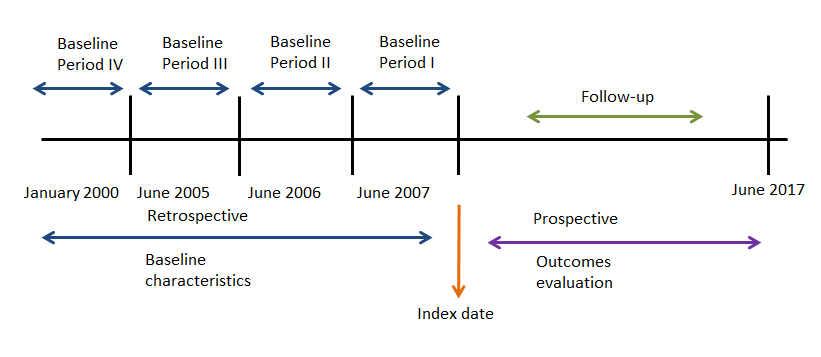
\includegraphics[width=\textwidth]{prelim-results/Panpredictor/timeline1.png}
			\caption{Study Design Timeline}
		\end{figure}
		
		Logically, model construction will encompass two steps: Using a sparsity inducing model to select among hundreds of variables, then building a model using the selected variables. In effect, algorithms will be chosen that perform both stages at once. See more details in the modeling section ahead.
		
		The covariates supplied to the first step will be: 
		\begin{itemize}
			\item Full demographic information, including age, sex, socioeconomic status, sector (arab/jew), ethnicity, etc.
			\item Clinical covariates, including blood pressure, height, weight, smoking status, etc. The data used will be the last result for each patient in the two years prior to the index date.
			\item Lab data, including all labs performed for each patient. Data will be extracted separately for the year before the index date, the year before that and the year before that.
			\item Chronic diagnoses, as defined by the Clalit's chronic registry\cite{Rennert2001}, up to the index date.
			\item Drug dispensings, including all drug dispensed to the patient in ATC4 granularity\cite{DrugStatisticsMethodology2010}. Data will be extracted separately for the 3 years before the index date and all the years before that.
		\end{itemize}
		A full list can be found in appendix C.
	
		\subsubsection{Part II}
		We will compare our models to four other models that encompass a large and representative sample of existing models, two designed to assess risk for cardiovascular disease (CVD) and two designed to assess risk  for mortality.
		
		The models with their respective populations and outcomes are:
		\begin{table}[H]
		\begin{tabular}{|p{4cm}|p{1cm}|p{3cm}|p{4cm}|}
			\hline
			Name & Age & Model & Outcome \\
			\hline
			American Heart Association 2013 pooled risk model\cite{Goff2014} & 40-79 & Cox proportional hazards & Myocardial infarction, coronary heart disease death, stroke and stroke death \\
			\hline
			Framingham general CVD risk score\cite{DAgostino2008} & 30-74 & Cox proportional hazards & CHD death, nonfatal MI, coronary insufficiency, stroke (ischemic or hemorrhagic), TIA, peripheral vascular disease, heart failure \\
			\hline
			Charlson Score\cite{Charlson1987} & 55-84 & Cox proportional hazards & All-cause mortality \\
			\hline
			QMortality\cite{Hippisley-Cox2017} & 65-100 & Cox proportional hazards & All-cause mortality \\
			\hline
		\end{tabular}
		\caption{Models to be Externally Validated}
		\end{table}
	
		Each model uses its own variables, see appendix A for full model variable lists.
		
		\subsubsection{Part III}
		The population for the application simulation will include all members of the Clalit's insured population as of 1/6/2007 that were members of the test set for the CVD prediction model. Inclusion and exclusion criteria will be the same as for the model (as mentioned above). The patients will be followed up for 10 years and their CVD outcomes recorded (as per the CVD outcomes in appendix A).
	
	\subsection{Data Extraction}
	The general population for all different parts of the study is the population of patients insured by Clalit Health Services (CHS). CHS is the largest sick fund in Israel, with an insured population of 4.4 active members. Clalit is both an insurer and a provider, directly providing primary care, specialist care, lab, imaging and pharamacy services. Additionally, clalit directly operates several large hospitals. The “attrition rate” (the percentage of patients leaving the sick fund each year) stands on a low 2\%, allowing long term follow-up of patients.
	
	The data will be collected using the CHS's electronic health record (EHR). CHS has maintained a comprehensive electronic health record since the year 2000, and has continued to improve it with time. This EHR contains, among others, demographic data, medical data (including clinical covariates, lab results, imaging studies, etc.) and claims data for both services rendered as part of the mandatory health insurance and for services rendered as part of the additive insurance (“Mashlim”). On top of the internal Clalit data, the database also contains external information such as the ministry of interior's causes of death listings and the ministry of health's cancer registry. This comprehensive database, combining both medical and claims data, covers large facets of a person's health.
	
	The difficulties that arise in conducting observational studies on EHR data are many and well documented: Data inaccuracy, missing data, cohort effects, selection biases, myriad ontologies, etc\cite{Hripcsak2011,Jensen2012,Goldstein2017}. Some of these issues, such as missing data, can be partially dealt with using statistical methods (see ahead), while some require in-depth expertise and know-how regarding the data's structure and collection methods, knowledge that can only be acquired through rigorous analysis of it. The Clalit's research institute's (CRI) is the research body for Clalit Health Services, and is thus the main consumer of the clalit's EHR data. This grants the CRI intimate knowledge of the data, as is evidenced by the many studies published in major journals based on the Clalit's database and on the CRI's methods in extracting its information (e.g. \cite{Reges2018,Dagan2017}).
	
	Data extraction principles for these studies are:
	\begin{itemize}
		\item Demographic characteristics will be extracted from the Clalit's demographic database. Those that are time-dependent (e.g. age) will be extracted current to the index dates, those that are constantly overridden will be extracted to their latest value (e.g. SES).
		\item Cause of death will be collected directly from the ministry of interior's causes of death table.
		\item Clinical covariates will be extracted from their dedicated database. The latest value prior to the index date will be used. Tests that can be used as-is (e.g. systolic blood pressure) will be used as-is. Weights and heights measured within a 3-month span will be joined for the calculation of BMI. Smoking status will be "flattened" to never/present/past to account for partial "pack-years" reporting.
		\item Lab data will be extracted from the dedicated lab results database, using the latest lab values prior to the index date.
		\item Diagnoses will be collected from the community (both session and permanent diagnoses), from hospitalizations and from the Clalit's chronic registry\cite{Rennert2001}. Diagnoses will be extracted based on ICD9 codes, ICPC codes and chronic registry codes. Community diagnoses will be corroborated using free text validation so as to exclude suspicions, etc.
		\item Drug dispensings will be evaluated using the dedicated pharmacy database. Actual dispensings will be counted (as opposed to prescriptions). Drug adherence will be calculated using drug prescriptions and drug dispensings, with PDC and MPR as the actual statistics\cite{Lam2015}.
		\item Health care utilization will be calculated by simply counting and summing the patient's encounters and actual cost, both in the community and in hospitals.
	\end{itemize}
	
	In part II, where external validation of international models is to take part, special care will be required to handle variables that are not perfect "fits" for the Clalit's database, for example:
	\begin{itemize}
		\item UK socioeconomic status ("Townsend Deprivation Score"), which has different levels and is directed in the opposite direction (more means lower SES) than the Clalit's socioeconomic status.
		\item Diagnoses, that are collected based on dedicated physician visits in cohort studies and on ICD codes in EHR based studies, will be collected using a mixture of ICD codes, free text validation and validation using lab measurements (e.g glucose for diabetes) and drug dispensings (e.g. diuretics, ACE inhibitors, beta blockers and calcium channel blockers for hypertension).
	\end{itemize}

	CVD definitions, that are used as the outcome in the different models, will be based on those defined by a consensus committee organized by the CRI and headed by a cardiology and neurology specialists. These definitions similar to those used outside the CRI, such as by the Israeli acute stroke registry\cite{ICDC2017} (active within the ICDC).
	
	\subsection{Descriptive Statistics}
	The specific population for each of the four models will be described in a dedicated population table ("Table 1") with appropriate statistics for each variable: proportions for categorical variables, means and standard deviations for continuous variables.
	
	The population to be used for comparing the external models to the internal model will also be described in a population table. This table will include separate columns for the train and test populations (see ahead for modeling details), with the same appropriate statistics for each variable. Statistical tests will be used to compare these populations for differences in baseline variables that could affect model generalizability. The statistical tests to be used are Student's t-test for continuous variables and the Chi square goodness-of-fit test for categorical variables, once the basic assumptions (e.g. normality) are tested.
	
	Missing data will be multiply imputed using chained equations. Specifically, continuous variables will be imputed using predictive mean matching, while categorical variables will utilize logistic regression\cite{Buuren2011}. Five datasets will be imputed, with the results combined as per Rubin's law\cite{Rubin1987}.
	
	\subsection{Modeling and Inferential Statistics}
	
		\subsubsection{Part I}
		
		To develop the new models we will create a generic framework capable of generating models for any disease, given a fitting definition of the outcome.
		
		The framework will serve two consecutive tasks. The first is to choose the relevant covariates from the long list of candidate covariates supplied to it. The second is to actually build the model.
		
		It should be specifically noted that both parts carry independent significance. The covariate selection awards biological insight into the risk factors for a disease, while the model is the actual tool used for risk prediction.
		
		The first step will involve applying a model to the training data that employs sparsity. That is, we will opt for models that include variable selection as a part of the fitting process. The hyperparameters for these models will be tuned using the validation set.
		
		The three sparsity inducing models we intend to fit are:
		\begin{enumerate}
			\item LASSO\cite{Tibshirani2011}
			\item Gradient Boosting\cite{Freund1997}
			\item Random Forest\cite{Breiman2001}
		\end{enumerate}
		
		least absolute shrinkage and selection operator (LASSO) is a variant of regression that adds a regularization term based on the $ L_1 $ norm of the coefficients to the normal loss function to be optimized. Namely, the model minimizes:
		
		\begin{equation*}
		\arg \min_w L(w) + \lambda \sum_{i}|\beta|_i
		\end{equation*}
		
		L being the likelihood function and lambda being a regularization parameter. Owing to the geometric structure of the $ L_1 $ norm, this has the effect of setting many covariates to 0, inducing sparsity. The parameter lambda is selected using cross-validation on the validation set, with predictive performance (e.g. AUROC) as the goal.
		
		As the regularization portion of the loss is dependent on variable scales, we will normalize the variables to have equal mean and standard deviation prior to model fitting.
		
		Gradient boosting is an ensemble method that combines several weak learners (e.g. shallow trees) together using a weighted majority vote. Each consecutive learning phase focuses on those samples in the training set that were predicted wrong by the previous phases.
		
		Random forest is also an ensemble method employing decision trees as the weak learners. It strives to induce variance among the trees by using bootstrapping to select the training set for each tree, and only using a randomly selected subset of features at each split in the tree.
		
		Both gradient boosting and random forest induce sparsity by deciding on the important features at each split in each tree. The rules for these decisions are themselves parameters to the models, but all generally employ a version of Claude Shannon's information entropy\cite{Shannon1948}:
		
		For a given variable x, the entropy is defined as $ H(x) = -\sum_{i=1}^{n} P(x_i) \log P(x_i)$. This entropy is maximized when the "doubt" about the value of a variable is maximal, and the different tree models strive to minimize it by choosing maximally informative variables for each split.
		
		Hyper-parameter tuning, per each model's hyper-parameter lists, will be conducted on the validation set using random search\cite{Bergstra2012}. The best performing model with regard to area under the ROC curve will be selected.
		
		We will include a learning curve for our model so as to demonstrate lack of over-fitting.
	
		\subsubsection{Part I}

		All externally validated models will be evaluated twice:
		\begin{enumerate}
			\item Once on a population that exactly mirrors the population they were originally defined on.
			\item Once on a common shared population that represents the population for which we intend to use the model in our thesis.
		\end{enumerate}
		This design is similar to previously published work\cite{Dagan2017}.
		
		The first phase will employ the full population matching the model's inclusion and exclusion criteria, so as to mirror their development population as much as possible.
		
		For the second phase we'll use only the inclusion and exclusion criteria detailed above. This will be a common, shared population so as to allow comparison of model's performance on a joint dataset.
		
		The population will be separated into three sets for the sake of model development: Train, Validation and Test in a 72\%/8\%/20\% ratio. The training and validation sets will be discussed in subsection "part II" ahead. The test set will be used for comparing model's performance.
		
		The following performance statistics will be computed and reported for each model\cite{Steyerberg2008,FrankE.Harrell2015}:
		
		\begin{itemize}
			\item Area under the receiver operating characteristics (AUROC) curve, or c-statistic, as a measure of discrimination.
			\item Calibration slope as a measure of calibration.
			\item Brier score, as a combined measure of prediction accuracy.
			\item Sensitivity, Specificity, PPV and NPV for the appropriate thresholds (e.g. 7.5\% for CVD prediction) as in existing guidelines\cite{Goff2014,Bibbins-Domingo2016}.
		\end{itemize}
		
		To calculate the risk scores, the exact coefficients as published by the model's authors will be used. If dedicated software is available, it will be used instead.
		
		Prior to comparing the model's to our own model, we will allow them linear recalibration, so as to "even the playing field" between a model being internally validated (our model) and models being externally validated. This recalibration will be done using the framework suggested by Van Houwlingen et al\cite{Houwelingen2000}. Specifically, the model's linear predictor will be fit again as a sole predictor in a logistic regression model and the ensuing slope and intercept recorded. These will then be used to adjust all model predictions.
	
		Mathematically:
		
		\begin{equation*}
		\forall_i \text{LP}_i = \sum_{j=1}^{p}\beta_jx_j
		\end{equation*}
		\begin{equation*}
		\hat{y}_i = \gamma \text{LP}_i + \delta
		\end{equation*}
		
		Where $ LP_i $ is the linear predictor, $ \beta_{ij} $ is the coefficient for covariate j in patient i, $ x_{ij} $ is the covariate j in patient i, $ \hat{y} $ is the recalibrated prediction, for which $ \gamma $ is the slope and $ \delta $ the intercept.
		
		Or in words: We take the linear predictor from the original model, but allow it a new slope and intercept, thus preserving the relative importance of each covariate in the model, with the freedom to reset the global risk.
	
		These models will be compared to the model as produced by the sparsity inducing algorithm (in step I) using the above mentioned performance measures. For the best performing CVD model, in preparation for step III, we will also include measures that demonstrate clinical utility, such as net reclassification improvement\cite{Pencina2008} and decision curves\cite{Vickers2016}.
		
		\subsubsection{Part III}
		We will use the both external CVD models and the internal CVD model to generate recommendations for statin and aspirin use for all patients in the test set of the CVD algorithm. We will illustrate that the internal model is more accurate when deciding on the population to treat, and its use would have prevented more CVD events.
		
	\section{Preliminary Results}
	We will present preliminary results for the first 2 parts.

	\subsection{Part 1}

	Population Table for the Framingham general CVD risk score\cite{DAgostino2008} model:

	\csvautotabular[separator=pipe]{prelim-results/FSRS/T1.csv}
	
	Calibration and ROC Curves for the Framingham general CVD risk score model are presented in appendix D.
	
	\subsection{Part 2}
	
	The population flow chart for the predictor is presented in appendix D.
	
	\section{References}
	
	%\nocite{*}
   	\printbibliography[heading=none]
   	
   	\newpage
   	\begin{appendices}
   		
   		\section{Model Variable Lists}
   		\begin{itemize}
   			\item American Heart Association 2013 pooled risk model
   			\begin{itemize}
   				\item Sex
   				\item Age
   				\item Total Cholesterol
   				\item HDL
   				\item Treated Systolic Blood Pressure
   				\item Untreated Systolic Blood Pressure
   				\item Smoking Status
   				\item Diabetes
   			\end{itemize}
   			\item Framingham general CVD risk score
   			\begin{itemize}
   				\item Sex
   				\item Age
   				\item Total Cholesterol
   				\item HDL
   				\item Treated Systolic Blood Pressure
   				\item Untreated Systolic Blood Pressure
   				\item Smoking Status
   				\item Diabetes
   			\end{itemize}
   			\item Charlson Score
   			\begin{itemize}
   				\item Myocardial Infarction
   				\item CHF
   				\item PVD
   				\item Cerebrovascular Disease
   				\item Dementia
   				\item Chronic Pulmonary Disease
   				\item Connective Tissue Disease
   				\item Ulcer Disease
   				\item Mild Liver Disease
   				\item Diabetes
   				\item Hemiplegia
   				\item Moderate or Severe Renal Disease
   				\item Diabetes with End Organ Damage
   				\item Any Tumor
   				\item Leukemia
   				\item Lymphoma
   				\item Moderate or Severe Liver Disease
   				\item metastatic Solid Tumor
   				\item AIDS
   			\end{itemize}
	   		\item QMortality
	   		\begin{itemize}
	   			\item Age
	   			\item Graphical Region
	   			\item Townsend Deprivation Score
	   			\item Ethnic Group
	   			\item Alcohol Intake
	   			\item Smoking Status
	   			\item BMI
	   			\item Unplanned Hospital Admissions
	   			\item Poor Mobility
	   			\item Lives in Care Home
	   			\item Lives Alone
	   			\item AF
	   			\item CHF
	   			\item CVD
	   			\item Valvular Heart Disease
	   			\item PVD
	   			\item Treated Hypertension
	   			\item CKD (stages 4 and 5)
	   			\item Diabetes
	   			\item Hypothyroidism
	   			\item Hyperthyroidism
	   			\item Cancer
	   			\item Chronic Liver Disease or Pancreatitis
	   			\item Malabsorption
	   			\item Peptic Ulcer
	   			\item Asthma or COPD
	   			\item Epilepsy
	   			\item Dementia
	   			\item Learning Disability
	   			\item Osteoporosis
	   			\item Fragility Fracture
	   			\item Parkinson's Disease or Syndrome
	   			\item RA
	   			\item Falls
	   			\item Bipolar Disease or Schizophrenia
	   			\item Depression in past 12 months
	   			\item VTE
	   			\item Anemia
	   			\item Abnormal LFTs
	   			\item High Platelet Count
	   			\item Leg Ulcer
	   			\item Blindness
	   			\item Appetite Loss in past 12 months
	   			\item Weight Loss in past 12 months
	   			\item Urinary Incontinence in past 12 months
	   			\item Nocturia in past 12 months
	   			\item Urinary Retention in past 12 months
	   			\item Syncope
	   			\item Dizziness in past 12 months
	   			\item Insomnia in past 12 months
	   			\item Dyspnea in past 12 months
	   			\item Hearing Impairment or deafness in past 12 months
	   			\item Loneliness in past 12 months
	   			\item Use of anticoagulants
	   			\item Use of antidepressants
	   			\item Use of antipsychotics
	   			\item Use of corticosteroids
	   			\item NSAIDs
	   		\end{itemize}
   		\end{itemize}
   		\newpage
   		
   		\section{Generic Predictor Variable List}
   		\begin{itemize}
   			\itemsep0em 
   			\item age
   			\item birth\_area\_desc
   			\item bmi\_last\_v
   			\item charlson
   			\item DBP\_last\_v
   			\item date\_of\_birth
   			\item date\_of\_death
   			\item ethnicity
   			\item GFR
   			\item immigration\_date
   			\item LEUCOCYTES-SED
   			\item ERYTHROCYTES-SED
   			\item EPITHELIAL-SED
   			\item BACTERIA-SED
   			\item ESTRADIOL (E-2)
   			\item PROGESTERONE
   			\item 17-OH-PROGESTERONE
   			\item LH
   			\item Throat culture p
   			\item FSH
   			\item WBC
   			\item PROLACTIN
   			\item TESTOSTERONE- TOTAL
   			\item Aerobic blood cult.
   			\item Anaerobic blood cult
   			\item Bacterial culture
   			\item Body fluid culture
   			\item Ear culture 1
   			\item Fungal culture
   			\item DHEA SULPHATE
   			\item MRSA culture
   			\item CORTISOL-BLOOD
   			\item Pediatric blood cul
   			\item Sputum culture
   			\item Stool culture
   			\item Throat culture
   			\item Urine dipsl culture
   			\item Urine culture
   			\item Urine plating cult.P
   			\item Wound culture
   			\item RBC
   			\item Wound and Sec.Aer+An
   			\item TSH
   			\item First isolate
   			\item Second isolate
   			\item PRELIMINARY
   			\item T3-TOTAL
   			\item T3- FREE
   			\item CPE culture result
   			\item T4- FREE
   			\item HB
   			\item PTH
   			\item HCT
   			\item PLT
   			\item MCV
   			\item MCH
   			\item MCHC
   			\item RDW
   			\item MPV
   			\item BAB- Blood agar base
   			\item MacConkey agar
   			\item Sabour dextrose agar
   			\item PCT
   			\item ESBL test
   			\item PDW
   			\item MID abs.
   			\item MID \%
   			\item VAR-F
   			\item LI
   			\item HDW
   			\item MICRO-F
   			\item ABO conf final (ad)
   			\item Rh confirmation
   			\item RH
   			\item BLOOD TYPE
   			\item Antibody screen Fin
   			\item BLAST-F
   			\item LUC\%
   			\item LUC abs
   			\item MPXI
   			\item LEFT SHIFT
   			\item MACRO\%
   			\item MICRO \%
   			\item HYPER\%
   			\item HYPO \%
   			\item ANISO-F
   			\item LYMP.abs
   			\item LYM\%
   			\item NEUT.abs
   			\item NEUT\%
   			\item MONO.abs
   			\item MONO\%
   			\item EOS.abs
   			\item EOS \%
   			\item BASO abs
   			\item BASO \%
   			\item HCT/HGB Ratio
   			\item Gram stain direct
   			\item Parasites microscopy
   			\item RDW-SD
   			\item RDW-CV
   			\item RETICUL. COUNT abs
   			\item RETICULOCYTES COUNT\%
   			\item ALY\%
   			\item ALY
   			\item LIC\%
   			\item LIC
   			\item P-LCR
   			\item CHr
   			\item CH
   			\item PLATLATE CLUMPS
   			\item MICRO\%/HYPO\%
   			\item NORMOBLAST.abs
   			\item NORMOBLAST.\%
   			\item TRANSGLUTAMINASE\_IgA
   			\item C13 UREA BREATH CALC
   			\item PT-INR
   			\item PT-SEC
   			\item PT \%
   			\item APTT-sec
   			\item APTT-R
   			\item FIBRINOGEN CALCU
   			\item FIBRINOGEN
   			\item CONTROL PT
   			\item CONTROL PTT
   			\item OCCULT BLOOD STOOL
   			\item LYMPHOCYTES \%-DIF
   			\item GLUCOSE
   			\item OCCULT BLOOD SCREEN
   			\item NEUTROPHILS\%-DIF
   			\item UREA
   			\item MONOCYTES\%-DIF
   			\item CREATININE
   			\item EOSINOPHILS\%-DIF
   			\item URIC ACID
   			\item BASOPHILS\%-DIF
   			\item SODIUM
   			\item POTASSIUM
   			\item CHLORIDE
   			\item CALCIUM
   			\item lab\_208512
   			\item PHOSPHORUS
   			\item CHOCOLATE
   			\item STABS \%-DIF
   			\item PROTEIN-TOTAL
   			\item ALBUMIN
   			\item ATYPICAL LYMPH.\%-DIF
   			\item CHOLESTEROL
   			\item LYMPHOCYTES abs-DIF
   			\item TRIGLYCERIDES
   			\item NEUTROPHILS abs-DIF
   			\item CHOLESTEROL- HDL
   			\item MONOCYTES abs-DIF
   			\item CHOLESTEROL-LDL calc
   			\item EOSINOPHILS abs-DIF
   			\item BASOPHILS abs-DIF
   			\item ALK. PHOSPHATASE
   			\item GOT (AST)
   			\item GPT (ALT)
   			\item STABS abs-DIF
   			\item GGT
   			\item LDH
   			\item ATYPICAL LYMPH-DIF
   			\item CK-CREAT.KINASE(CPK)
   			\item ANISOCYTOSIS-DIF
   			\item AMYLASE
   			\item IRON
   			\item TRANSFERRIN
   			\item BILIRUBIN TOTAL
   			\item BILIRUBIN-DIRECT
   			\item ALBUMIN (BY EP)
   			\item GLOBULIN ALPHA-1
   			\item GLOBULIN ALPHA-2
   			\item GLOBULIN GAMA
   			\item REMARK-MANU-DIF
   			\item MAGNESIUM
   			\item HEMOGLOBIN A1C \%
   			\item FRUCTOSAMINE
   			\item SODIUM
   			\item POTASSIUM
   			\item CHLORIDE
   			\item CALCIUM IONIZED
   			\item pH BLOOD
   			\item pCO2
   			\item TOTAL HEMOGLOBIN
   			\item HCO3
   			\item TCO2
   			\item pO2
   			\item O2 SATURATION
   			\item Hct- OXIMETRY
   			\item CARBOXYHEMOGLO-OXIME
   			\item DEOXYHEMOGLOBIN-OXIM
   			\item METHEMOGLOBIN-OXIMET
   			\item OXYHEMOGLOBIN-OXIMET
   			\item STD BASE EXC (SBE)
   			\item TOTAL OXYGEN CONTENT
   			\item O2 TEN. AT 50\% SAT
   			\item ACTUAL BASE EXCBSS
   			\item STANDARD BICARBONATE
   			\item LACTATE
   			\item VITAMIN B12
   			\item VITAMIN D (25-OH)
   			\item LIPASE
   			\item BILIRUBIN-NEONATAL
   			\item ZINC
   			\item REMARK-MAN-DIF
   			\item TROPONIN I
   			\item TROPONIN T
   			\item FOLIC ACID
   			\item CHOLESTEROL/ HDL
   			\item TRANSFERRIN SATURATI
   			\item MICROALBUMIN/CREAT
   			\item GLUCOSE I
   			\item BILIRUBIN INDIRECT
   			\item IRON SATURATION
   			\item GLOBULIN
   			\item ICTERIC
   			\item HEMOLYTIC
   			\item LIPEMIC
   			\item VLDL
   			\item ESR
   			\item CREATININE- U 24h
   			\item PROTEIN- U SAMPLE
   			\item CREATININE- U SAMPLE
   			\item SODIUM-URINE SAMPLE
   			\item POTASSIUM- U SAMPLE
   			\item CALCIUM- URINE 24h
   			\item PROTEIN- URINE 24h
   			\item MICROALBUMIN- U 24h
   			\item CALCIUM- U SAMPLE
   			\item MICROALBUMIN-U SAMP
   			\item HbF
   			\item HbA2
   			\item CARBAMAZEPINE
   			\item DIGOXIN
   			\item VALPROIC ACID
   			\item GLUCOSE 50g
   			\item CREATININE ENZ.CHILD
   			\item GLOM.FILTR.RATE
   			\item NON-HDL\_CHOLESTEROL
   			\item ANA PATTERN
   			\item ANA TITER
   			\item CELIAC SCREEN
   			\item ANTISTREPTOLYSIN O
   			\item C-REACTIVE PROTEIN
   			\item RHEUMATOID FACTOR
   			\item ANTINUCLEAR Ab\_(ANA)
   			\item ANTI CARDIOLIPIN IgM
   			\item THYROGLOBULIN Ab
   			\item DNA (ds) Ab
   			\item RNP
   			\item Sm (anti Smith Ab)
   			\item COMPLEMENT C3
   			\item COMPLEMENT C4
   			\item TOXOPLASMA IgG
   			\item TOXOPLASMA IgM
   			\item HELICO PYLORI IgG
   			\item REMARKS (GENERAL)
   			\item REMARKS MICRO
   			\item HEPATITIS Bs Ag
   			\item HEPATITIS C Ab
   			\item HEPATITIS Bs Ab
   			\item HEPATITIS A IgM
   			\item CMV IgG
   			\item CMV IgM
   			\item EBV VCA\_IgG
   			\item EBV IgG-EBNA
   			\item EBV VCA IgM
   			\item RUBELLA Ab IgG
   			\item Anti Jo-1 Ab
   			\item Scl-70 Ab
   			\item ANTI CARDIOLIPIN IgG
   			\item HEPATITIS Bc Ab TOT.
   			\item Ig-E TOTAL
   			\item ANTI THYROID PEROXID
   			\item COOMBS INDIRECT
   			\item IgG
   			\item IgM
   			\item IgA
   			\item ANTICENTROMERE Ab
   			\item ALPHA FETOPROTEIN TM
   			\item CA-125
   			\item CA-15-3
   			\item CA-19-9
   			\item CEA
   			\item FERRITIN
   			\item PSA
   			\item GLUCOSE - U STRIP
   			\item BILIRUBIN- U STRIP
   			\item KETONES- U STRIP
   			\item SPECIFIC GRAV-U STRI
   			\item PROTEIN- U STRIP
   			\item NITRITE- U STRIP
   			\item LEUCOCYTES - U STRIP
   			\item ERYTHROCYTES-U STRIP
   			\item UROBILINOGEN-U STRIP
   			\item PH- U STRIP
   			\item SBP\_last\_v
   			\item sector
   			\item SES
   			\item sex
   			\item smoking\_last\_v
   			\item sw\_confined
   			\item sw\_immigrant
   			\item sw\_malig\_active
   			\item sw\_malig\_ever
   			\item sw\_nursing\_care
   			\item Antiinfectives for Local Oral Treatment
   			\item Corticosteroids for Local Oral Treatment
   			\item Calcium Compounds
   			\item Combination of Complexes of Calcium, Magnesium and AluminumCompounds
   			\item H2 Receptor Antagonists
   			\item Proton Pump Inhibitors
   			\item Synthetic Anticholinergics, Esters with Tertiary Amino Groups
   			\item Papaverine and Derivatives
   			\item Other drugs for func. gastro. disorders
   			\item Other Antispasmodics in Combination with Analgesics
   			\item Propulsives
   			\item Serotonin (5HT3) Antagonists
   			\item Other Antiemetics
   			\item Bile Acid and derivatives
   			\item Softeners, Emollients
   			\item Contact Laxatives
   			\item Osmotically Acting Laxatives
   			\item Enemas
   			\item Other drugs for constipation
   			\item Charcoal Preparations
   			\item Bismuth Preparations
   			\item Oral Rehydrating Salt Formulations
   			\item Antipropulsives
   			\item Aminosalicylic Acid and Similar Agents
   			\item Antidiarrheal Microorganisms
   			\item Enzyme Preparations
   			\item Insulins and Analogues, for Injection, Fast Acting
   			\item Insulin and Analogues, for Injection, Long Acting
   			\item Biguanides
   			\item Sufonylureas
   			\item Combinations or Oral Blood Glucose Lowering Drugs
   			\item Alpha Glucosidase Inhibitors
   			\item Dipeptidyl peptidase 4 (DPP-4) Iinhibi.
   			\item Glucagon-like peptide-1(GLP-1) analogues
   			\item Sodium-glucose co-transfer 2(SGLT2) Inhibitors
   			\item Other Blood Glucose Lowering Agents, Excluding Insulins
   			\item Multiple Vitamins with Minerals
   			\item Vitamin D and Analogues
   			\item Vitamin B1, in Combination with Vitamin B6 and/or B12
   			\item Ascorbic Acid (Vitamin C), Plain
   			\item Ascorbic Acid (Vitamin C), Combinations
   			\item Other Plain Vitamin Combinations
   			\item Vitamins, Other Combinations
   			\item Calcium
   			\item Calc.,Comb.with vit.D and/or other drugs
   			\item Potassium
   			\item Magnesium
   			\item Varoius Alimentary Tract and Metabolism Products
   			\item Vitamin K Antagonists
   			\item Heparin Group
   			\item Platelet Aggregation Inhibitors, Excluding Heparin
   			\item Direct Thrombin Inhibitors
   			\item Direct factor Xa inhibitors
   			\item Iron Bivalent, Oral Preparations
   			\item Iron Trivalent, Oral Preparations
   			\item Iron , Parenteral Preparations
   			\item Iron in Combination with Folic Acid
   			\item Iron in Other Combinations
   			\item Vitamin B12 (Cyanocobalamine and Derivatives)
   			\item Folic Acid and Derivatives
   			\item Other Antianemic Preparations
   			\item Digitalis Glycosides
   			\item Antiarrhythmics, Class IC
   			\item Antiarrhythmics, Class III
   			\item Organic Nitrates
   			\item Imidazoline Receptor Agonists
   			\item Alpha Adrenergic Blocking Agents
   			\item Thiazides, Plain
   			\item Sulfonamides, Plain
   			\item Aldosterone Antagonists
   			\item Other Antihemorrhoidals for Topical Use
   			\item Beta Blocking Agents, Non Selective
   			\item Beta Blocking Agents, Selective
   			\item Alpha and Beta Blocking Agents
   			\item Dihydropyridine Derivatives
   			\item Phenylalkalylamine Derivatives
   			\item ACE Inhibitors, Plain
   			\item ACE Inhibitors and Diuretics
   			\item ACE Inhibitors and Calcium Channel Blockers
   			\item Angiotensin II Antagonists, Plain
   			\item Angiotensin II Antagonists and Diuretics
   			\item Angiotensin II Antagonists and Calcium Channel Blockers
   			\item HMG CoA Reductase Inhibitors
   			\item Fibrates
   			\item Other lipid modifying agents
   			\item Imidazole Derivatives
   			\item Other Antifungals for Topical Use
   			\item Antifungals for Systemic Use
   			\item Zinc Products
   			\item Soft Paraffin and Fat Products
   			\item Carbamide Products
   			\item Salicylic Acid Products
   			\item Other Emollients and Protectives
   			\item Protectives Against UV-Radiations for Topical Use
   			\item Cod Liver Oil Ointments
   			\item Other Cicatrizants
   			\item Antihistamines for Topical Use
   			\item Anesthetic for Topical Use
   			\item Other Antipsoriatics for Topical Use
   			\item Other Antibiotics for Topical Use
   			\item Sulfonamides
   			\item Antivirals
   			\item Corticosteroids, Potent (Group III)
   			\item Corticosteroids, Very Potent (Group IV)
   			\item CORTICOSTEROIDS, WEAK, COMBINATIONS WITH ANTIBIOTICS
   			\item CORTICOSTEROIDS, MODERATELY POTENT, COMBINATIONS WITH ANTIBITICS
   			\item Corticosteroids, Potent, Combinations with Antibiotics
   			\item Corticosteroids, Potent, Other Combinations
   			\item Biguanides and Amidines
   			\item Phenol and Derivatives
   			\item Iodine Products
   			\item Other Antiseptics and Disinfectants
   			\item Retinoids for Topical Use in Acne
   			\item Peroxides
   			\item Antiinfectives for Treatment of Acne
   			\item Retinoids for Treatment of Acne
   			\item Medicated Shampoos
   			\item Wart and Anti-Corn Preparations
   			\item Other Dermatologicals
   			\item Imidazole Derivatives
   			\item Progestogens and Estrogens, Fixed Combinations
   			\item Progestogens
   			\item 3-Oxoandrosten (3) Derivatives
   			\item Natural and Semisynthetic Estrogens, Plain
   			\item Pregnen (4) Derivatives
   			\item Estren Derivatives
   			\item Progestogedns and Estrogens in Fixed Combination
   			\item Gonadotrophins
   			\item Antiandrogens and Estrogens
   			\item Selective Estrogen Receptor Modulator
   			\item Acidifiers
   			\item Urinary Concrement Solvents
   			\item Drugs for urinary frequency and incontinence
   			\item Drugs Used in Erectile Dysfunction
   			\item Other Urologicals
   			\item Alpha-Adrenoreceptor Antagonists
   			\item Testerone-5 Alpha Reductase Inhibitors
   			\item Other Drugs Used to Treat Benign Prostatic Hypertrophy
   			\item Somatotrophin and Somatrophin Agonists
   			\item Vasopressin and Analogues
   			\item Glucocorticoids
   			\item Thyroid Hormones
   			\item Other anti-parathyroid agents
   			\item Tetracyclines
   			\item Penicillins with Extended Spectrum
   			\item Beta Lactamase Sensitive Penicillins
   			\item Combinations of Penicillins, Including Beta-Lactamase Inhibitors
   			\item First-Generation Cephalosporins
   			\item Second-Generation Cephalosporins
   			\item Combinations of Sulfonamides and Trimethoprim, Including Derivatives
   			\item Macrolides
   			\item LINCOSAMIDES
   			\item Fluoroquinolones
   			\item Nitrofuran Derivatives
   			\item Other Antibacterials
   			\item Triazole Derivatives
   			\item Nucleosides and Nucleotides (excl. Reverse Transcriptase Inhibitors)
   			\item Antivirals for treatment of HIV infections, combinations
   			\item Influenza Vaccines
   			\item Hepatitis Vaccines
   			\item Bacterial and Viral Vaccines, Combined
   			\item Pyrimidine Analogues
   			\item Monoclonal Antibodies
   			\item Other Antineoplastic Agents
   			\item Gonadotrophin Releasing Hormone Analogues
   			\item Antiestrogens
   			\item Aromatase inhibitors
   			\item SELECTIVE IMMUNOSUPPRESANTS
   			\item Tumor Necrosis Factor Alpha (TNBF-a) Inhibitors
   			\item Calcineurin Inhibitors
   			\item Other Immunosuppressants
   			\item Acetic Acid Derivatives and Related Substances
   			\item Oxicams
   			\item Propionic Acid Derivatives
   			\item Coxibs
   			\item Other Antiinflammatory and Antirheumatic Products, Non Steroids
   			\item Antiinflammatory Preparations, Non Steroid for Topical Use
   			\item Capsicum and Similar Agents
   			\item Preparations with Salicylic Acid Derivatives
   			\item Ethers, Chemically Close to Antihistamines
   			\item Other Centrally Acting Agents
   			\item Preparations Inhibiting Uric Acid Production
   			\item Preparations with No Effect on Uric Acid Metabolism
   			\item Biphosphonates
   			\item Biphosphonates and Calcium, Sequential Preparations
   			\item Amides
   			\item Natural Opium Alkaloids
   			\item Phenylpiperidine Derivatives
   			\item Oripavine Derivatives
   			\item Opioids in combin. with non-opioid analg.
   			\item Other Opioids
   			\item Pyrazolones
   			\item Anilides
   			\item SELECTIVE 5HT-RECEPTOR AGONISTS
   			\item Barbiturates and Derivatives
   			\item Hydantoins and Derivatives
   			\item Benzodiazepine Derivatives
   			\item Carboxamide Derivatives
   			\item Fatty Acid Derivatives
   			\item Other Antiepileptics
   			\item Tertiary Amines
   			\item DOPA and DOPA Derivatives
   			\item Amantane Derivatives
   			\item Dopamine Agonists
   			\item Monoamine Oxidase Type B Inhibitors
   			\item Phenothiazines with Aliphatic Side Chain
   			\item Phenothiazines with Piperazine Structure
   			\item Phenothiazines with Piperidine Structure
   			\item Butyrophenone Derivatives
   			\item Thioxanthine Derivatives
   			\item Dibenzepines, Oxazepines, thiazepines, and oxepines
   			\item Benzamides
   			\item Lithium
   			\item Other Antipsychotics
   			\item Benzodiazepine Derivatives
   			\item Benzodiazepine Derivatives
   			\item Benzodiazepine Related Drugs
   			\item Other Hypnotics and Sedatives
   			\item Nonselective Monoamine Reuptake Inhibitors
   			\item Selective Serotonin Reuptake Inhibitors
   			\item Other Antidepressants
   			\item Centrally Acting Sympathomimetics
   			\item Anticholinesterases
   			\item Other Anti-Dementia Drugs
   			\item Drugs Used in Nicoitine Dependence
   			\item Antivertigo Preparations
   			\item Nitroimidazole Derivatives
   			\item Aminoquinolines
   			\item Benzimidzole Derivatives
   			\item Other Ectoparasiticides, Including Scabies
   			\item Other Insecticides and Repellants
   			\item Sympathomimetics, Plain
   			\item Sympathomimetics, Combinations Excluding Corticosteroids
   			\item Corticosteroids
   			\item Other Nasal Preparations
   			\item Sympathomimetics
   			\item Antiseptics
   			\item Selective Beta-2 Adrenoreceptor Agonists
   			\item Adrenergics in combinations with corticosteroids or other drugs, excl. anticholinergics
   			\item Corticosteroids
   			\item Anticholinergics
   			\item Leukotriene Receptor Antagonists
   			\item Expectorants
   			\item Mucolytics
   			\item Opium Alkaloids and Derivatives
   			\item Other Cough Suppressants
   			\item Opium Derivatives and Expectorants
   			\item Substituted Alkylamines
   			\item Phenothiazine Derivatives
   			\item Piperazine Derivatives
   			\item Other Antihistamines for Systemic Use
   			\item ANTIBIOTICS
   			\item Fluoroquinolones
   			\item Corticosteroids, Plain
   			\item Corticosteroids and Antiinfectives in Combination
   			\item Sympathomimetics in Glaucoma Therapy
   			\item Carbonic Anhydrase Inhibitors
   			\item Beta Blocking Agents
   			\item Prostaglandin Analogues
   			\item Sympathomimetics Used as Decongestants
   			\item Other Antiallergics
   			\item Other Ophthalmologicals
   			\item Corticosteroids and Antiinfectives in Combination
   			\item Analgesics and Anesthetics
   			\item Indifferent Preparations
   			\item Antiinfectives
   			\item Drugs for Treatment of Hyperkalemia
   			\item Nutrients with Low Calcium Content
   			\item Other Infant Formulas
   			\item Fat/Carbohydrate/Protein/Minerals/Vitamins, Combinations
   			\item Solvents and Diluting Agents, Including Irrigating Solutions
   			\item Cosmetics-C
   			\item Cosmetics-E
   			\item Hearing loss and Deafness
   			\item S - IHD (s/p MI)
   			\item S - Ischemic Heart Disease
   			\item Valvular Cardiac Dis (excl. MVP)
   			\item CHF-systolic w/o selected medications
   			\item CHF-systolic with selected medications
   			\item CHF-non systolic
   			\item CHF NOS with diuretics
   			\item CHF NOS
   			\item Cardiomyopathy
   			\item IHSS
   			\item Atrial fibrilation
   			\item Arrhythmia other
   			\item S - Hypertension / Diet Treatment
   			\item S - Hypertension / Drug Treatment
   			\item S - Hypertension / Unknown Treatment
   			\item Pulmonary Hypertension
   			\item s/p CVA
   			\item Carotid Artery Disease
   			\item S - Diabetes PVD
   			\item S - PVD
   			\item Aortic Aneurism
   			\item S - Amputation of Limb (Diabetic)
   			\item Amputation of Limb (Non-Diabetic)
   			\item S - Amputation of Limb
   			\item COPD
   			\item S - Asthma
   			\item s/p Pulmonary Embolism
   			\item s/p Pneumothorax
   			\item Chronic Bronchitis
   			\item Bronchiectasis
   			\item Hepatitis B Carrier
   			\item Celiac Disease
   			\item Peptic Ulcer
   			\item Reflux Esophagitis / Gastritis / Deudenitis
   			\item Irritable Bowel Syndrome
   			\item Addisons Disease
   			\item Chronic Act/Per Hepatitis
   			\item Cirrhosis
   			\item Wilsons Disease
   			\item Other Liver Disease
   			\item Ulcerative Colitis
   			\item Crohns Disease
   			\item H - Dialysis
   			\item Kidney Transplant
   			\item Prostatic Hypertrophy
   			\item Liver Transplant
   			\item Heart Transplant
   			\item Pancreas Transplant
   			\item Lung Transplant
   			\item Bone Marrow Transplant
   			\item Other Transplant
   			\item Unknown Transplant
   			\item Chronic Renal Failure
   			\item s/p splenectomy
   			\item Infertility Male/Female
   			\item S - Diabetic Nephropathy
   			\item S - Other Kidney Disease
   			\item Hepatitis C Carrier
   			\item Pemphigus Vulgaris
   			\item Psoriasis
   			\item Hidradenitis Suppurativa
   			\item Arthropathy
   			\item SLE
   			\item Rheumatoid Arthritis
   			\item Osteoporosis
   			\item Joint Replacement
   			\item Sarcoidosis
   			\item Scleroderma
   			\item Behcets Disease
   			\item Other Rheumatic / Autoimmune
   			\item Polymyalgia Rheumatica
   			\item Gout
   			\item s/p Head of Femur Fracture
   			\item Congenital Anomalies
   			\item H - AIDS Patient
   			\item HIV Carrier
   			\item Familial Mediteranean Fever
   			\item G-6-P-D Deficiency
   			\item Amyloidosis
   			\item S - Breast Cancer
   			\item S - Malignancy of Colon or Rectum
   			\item S - Malignancy of Prostate
   			\item S - Malignancy of Lung
   			\item S - Malignancy of Bladder
   			\item S - Malignancy of Ovary
   			\item S - Malignancy of Uterus
   			\item S - Malignancy of Pancreas
   			\item S - Malignancy of Brain / CNS
   			\item S - Stomach Cancer
   			\item S - Melanoma
   			\item S - Hodgkins Lymphoma
   			\item S - Non Hodgkin Lymphoma / Mycosis Fungoides
   			\item S - Acute Leukemia
   			\item S - Chronic Leukemia
   			\item S - Malignancy of Kidney
   			\item S - Malignancy of Larynx
   			\item S - Malignancy of Cervix Uteri
   			\item S - Malignancy of Pharynx
   			\item S - Malignancy of Esophagus
   			\item S - Malignancy of Liver / Bile Ducts
   			\item S - Malignancy of Thyroid
   			\item S - Malignancy of Bone
   			\item S - Malignancy of Connective Tissue / Sarcoma
   			\item S - Malignancy of Other Male/Female Genital Organs
   			\item S - Multiple Myeloma
   			\item S - Polycytemia Vera
   			\item S - Myelodysplastic Syndrom
   			\item S - Myelo/Lymphoproliferative Syndrom
   			\item S - Neurofibromatosis
   			\item S - Malignancy of Other Sites
   			\item S - Malignancy of Unknown Site
   			\item Tuberculosis
   			\item Benign Brain Tumor
   			\item Disability / Bedbound
   			\item Disability / Homebound
   			\item Disability / Requires assistance with ambulation
   			\item Breast Family History
   			\item Colon Family History
   			\item Hyperthyroidism
   			\item Hypothyroidism
   			\item Tuberculosis s/p
   			\item S - Diabetes / Diet Treatment
   			\item S - Diabetes / Oral Treatment
   			\item S - Diabetes / Insulin Treatment
   			\item S - Diabetes / Insulin + Oral Treatment
   			\item S - Diabetes / Unknown Treatment
   			\item H - Gaucher Disease
   			\item Hypo/Hyperparathyroidism
   			\item Acromegaly
   			\item Obesity
   			\item S - Hyperlipidemia / No Treatment
   			\item S - Hyperlipidemia / Treatment
   			\item S - Hyperlipidemia / Unknown Treatment
   			\item Cystic Fibrosis
   			\item Hyperprolactinemia
   			\item Other Endocrine and Metabolic Disease
   			\item Syphilis / Gonorrhea
   			\item Cushings Disease
   			\item Diabetes Insipidus
   			\item Hypophysary Adenoma
   			\item H - Hemophilia
   			\item H - Thalassemia Minor
   			\item H - Thalassemia Intermedia
   			\item H - Thalassemia Major
   			\item H - Thalassemia NOS
   			\item Other Hematologic Dis (excl. Iron Def Anemia)
   			\item Sickle Cell Anemia
   			\item Pernicious Anemia
   			\item ITP
   			\item Psychoses
   			\item Schizophrenia
   			\item Bipolar Disease (Manic Depressive)
   			\item Autism
   			\item Neuroses
   			\item Depression
   			\item Anxiety
   			\item Eating Disorders
   			\item Alcohol Abuse
   			\item Current Smoker
   			\item Former Smoker
   			\item Smoker
   			\item Drug Abuse
   			\item Mental Retardation (incl. Down)
   			\item Dementia / Alzheimers / OMS
   			\item Myasthenia Gravis
   			\item Parkinsons Disease
   			\item Epilepsy
   			\item Multiple Sclerosis
   			\item Cerebral Palsy
   			\item Huntingtons Chorea
   			\item Familial Dysautonomia
   			\item Hereditary Neurological Disease
   			\item Muscular Dystrophy
   			\item Motor Neuron Disease
   			\item S - Diabetic Neuropathy
   			\item s/p TIA
   			\item S - Other Neurological Disease
   			\item S - Diabetic Retinopathy
   			\item Non-Diabetic Retinopathy
   			\item S - Retinopathy
   			\item Glaucoma
   			\item Blindness
   			\item Retinitis Pigmentosum
   			\item Chronic Medication User
   		\end{itemize}
   		\newpage
   		
   		\section{Preliminary Result Graphs and Drawings}
   			\subsection{Framingham CVD Risk Score Result Graphs}
	   		\begin{figure}[H]
	   			\begin{minipage}{.45\linewidth}
	   				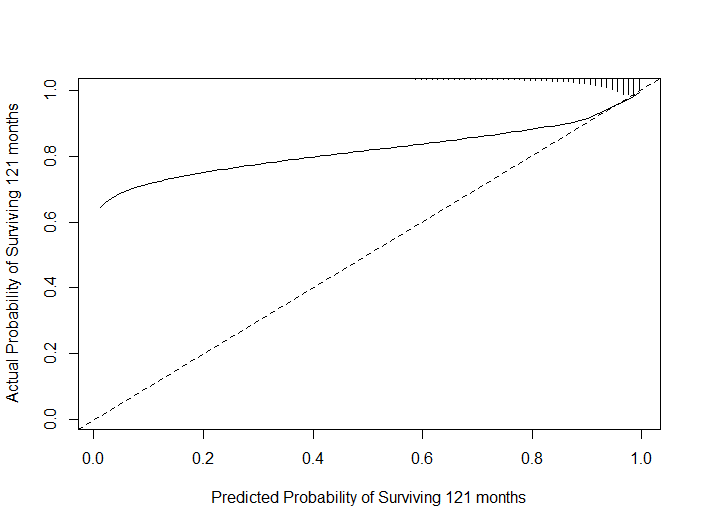
\includegraphics[width=8cm, height=8cm]{prelim-results/FSRS/FSRScal.png}
	   				\label{Fram1}
	   				\captionsetup{justification=justified,singlelinecheck=false,margin=1cm}
	   				\caption{Framingham Calibration Curve}
	   			\end{minipage}
	   			\hspace{.01\linewidth}
	   			\begin{minipage}{.45\linewidth}
	   				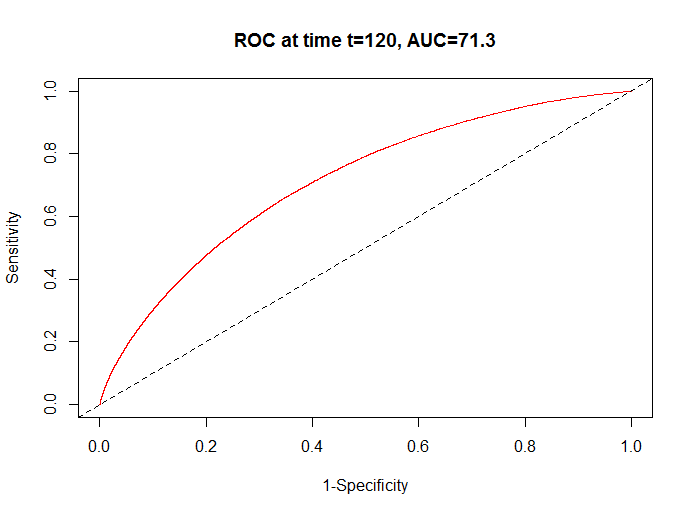
\includegraphics[width=8cm, height=8cm]{prelim-results/FSRS/FSRSdisc.png}
	   				\label{Fram2}
	   				\captionsetup{justification=justified,singlelinecheck=false,margin=1cm}
	   				\caption{Framingham ROC Curve}
	   			\end{minipage}
	   		\end{figure}
   		
   			\subsection{Clalit Model Population Flow Chart}
   			\begin{figure}[H]
	   			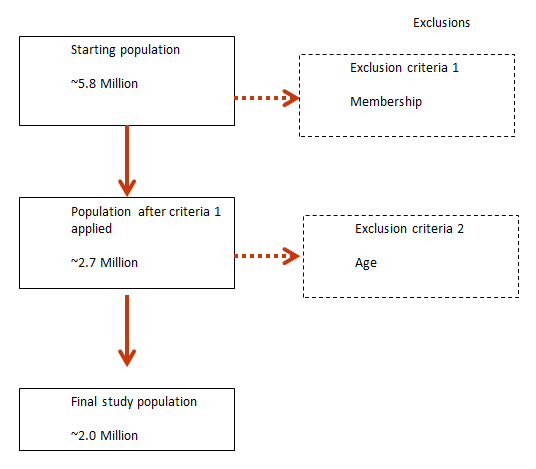
\includegraphics[width=10cm,height=8cm]{prelim-results/Panpredictor/pop_flow_chart.png}
	   			\captionsetup{justification=justified,singlelinecheck=false,margin=2cm}
	   			\caption{Population Flow Chart}
	   		\end{figure}
   			
   	\end{appendices}
	
\end{document}